\documentclass[a4paper, 11pt]{report}

\usepackage{microtype}
\usepackage{graphicx}
\usepackage{wrapfig}
\usepackage[utf8]{inputenc}
\usepackage[T1]{fontenc}
\usepackage{lmodern}
\usepackage{listings}

\makeatletter

\title{\LARGE{\textbf{CS 118 Project 1 Report}}\\
Web Server Implementation using BSD Sockets}
\author{\textsc{Yukai Tu 204761085}
\\\textsc{Xufan Wang 204477479}}
\date{\today}

\begin{document}


\maketitle

\section*{Introduction}

For this project, we implemented a web server in C using the BSD socket programming library on a 32-bit Ubuntu Virtual machine. The server implementation include two parts. For part A, the server can receive HTTP requests and then dump request messages to the console. For part B, one more functionality is added to the server, so that it can further parse the requests, generate HTTP response messages consisting of the requested files preceded by header lines, and send the responses back to the client.

%------------------------------------------------

\section*{Compilation and Usage}

Tester can use the following steps to compile the server.
\scriptsize
{\fontfamily{qcr}\selectfont
\mbox{}\\
\indent1. Navigate to the directory containing the source files. \\
\indent2. Run the command "make".\\
\indent2. Run the command "chmod +x serverFork".\\
}
\normalsize
After compilation, use the command:
\scriptsize
{\fontfamily{qcr}\selectfont
\mbox{}\\
\indent./serverFork <portnum>\\
}
\normalsize
to start the server. In the above command, <portnum> is a port number that the server will bind to, so the same port should be used for the client to send request.\\
After the server starts, the client can connect to the server by accessing following URL using a web browser.
\scriptsize
{\fontfamily{qcr}\selectfont
\mbox{}\\
\indent http://<machine name>:<portnum>/<html file name>\\
}
\normalsize
In the above command, <machine name> should be the name of the server machine, and <html file name> should be the name of a file that the client would like to receive.

%------------------------------------------------

\section*{High-Level Description}
For both Part A and Part B, the server builds a communication point through a port by using functions in the libraries:

\begin{lstlisting}[language=C]
#include <sys/types.h>
#include <sys/socket.h>
#include <netinet/in.h>
\end{lstlisting}

\noindent which define different data structures and socket operations.\\\\
To be more specific, the server first use the {\fontfamily{qcr}\selectfont socket} function to create a socket. It then uses the function {\fontfamily{qcr}\selectfont bind} to bind the new socket to a port on the local machine. The port number is specified by the user.
After doing those, the server starts listen to the socket for any client requests, and this is done by using {\fontfamily{qcr}\selectfont listen} function. By now, the socket is ready and requests can be sent through it by the client.\\\\

\noindent The server accepts requests with the function {\fontfamily{qcr}\selectfont accept}. To keep the server ready to accept new requests, once the server receive a request, it will fork a child process to serve the request, so that the parent process can continue to run {\fontfamily{qcr}\selectfont accept} and wait for the next request. When the child exits, the parent handles the signal {\fontfamily{qcr}\selectfont SIGCHILD} to prevent zombie processes.\\\\

\noindent As the child process is forked, it starts to parse the request, send console outputs and responses, and exit when all the work is finished for that request. It mainly runs two functions, {\fontfamily{qcr}\selectfont parseRequest} and {\fontfamily{qcr}\selectfont serveRequest}.\\\\

\noindent The dumping functionality in part A is implemented in {\fontfamily{qcr}\selectfont parseRequest} function:

\begin{lstlisting}[language=C]
void parseRequest(int sock, RequestHeader* header);
\end{lstlisting}

\noindent It first read the request through socket file descriptor {\fontfamily{qcr}\selectfont sock} into a buffer, then print out the content of the buffer, which is a request line followed by several header lines. It also extract the header of the request and store it into {\fontfamily{qcr}\selectfont header}. This header is used for part B.\\\\

\noindent The functionality of sending response in part B is implemented in the {\fontfamily{qcr}\selectfont serveRequest} function:

\begin{lstlisting}[language=C]
void serveRequest(int sock, const RequestHeader header);
\end{lstlisting}

\noindent The function tries to read the file specified in {\fontfamily{qcr}\selectfont header}. If the file does not exist or it cannot be opened, it will send an error message to inform the client. If the file exists, the server will send an HTTP response message, with the file included, to the client. The server determines the MIME type of the requested file by looking at the URI in the header, and generate different response messages accordingly.

%------------------------------------------------

\section*{Difficulties}

The main difficulty of this project lies in the formatting of response messages. Based on RFC 1945, the header can include many header lines. It took us some time to figure out which ones should be included in the header and which should not.\\\\

\noindent Also, we tried many ways to parse the header of request messages. We are currently using the function {\fontfamily{qcr}\selectfont strtok}, which splits the buffer by delimiter to accomplish this, since the function uses only a few lines. However, since the function will change the original buffer, it can only be used to parse the first header line. The method is sufficient but not elegant enough.\\\\

\noindent Another difficulty would be that when we tried to send images to the browser, we always get "CONTENT LENGTH ERR". We debugged the code which gets the length of the content, but we eventually found out that the bug is cause by the wrong buffer size of the response message.

%------------------------------------------------

\section*{Sample Output}

After starting the server, we can send requests to the server by a browser. Here is the sample output from the request:
\scriptsize
{\fontfamily{qcr}\selectfont
\mbox{}\\
\indent http://192.168.130.148:8082/test.html>
}
\normalsize

\noindent In which, "test.html" is an HTML file which refers to a JPEG file and a GIF file. On the client side, the output appears to be:

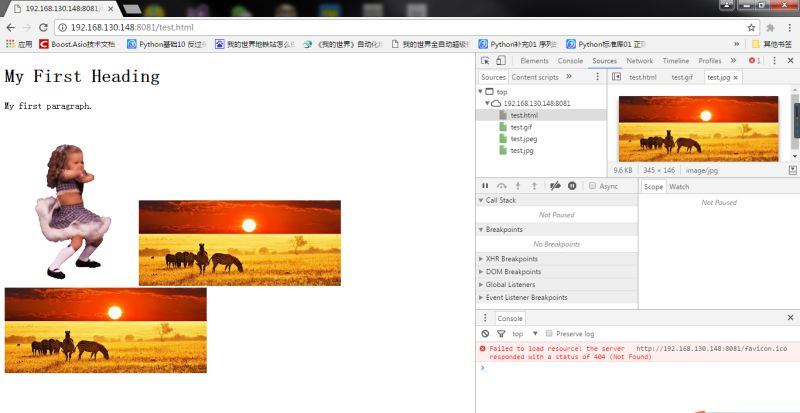
\includegraphics[scale=0.54]{client_output.jpg}

\noindent On the right side, we can see that the HTML file actually refers to three files, and they are all displayed correctly on the left side, in the HTML format.\\\\

\noindent At the server side, the console displays the message contents of four requests. The first one is for the HTML file.

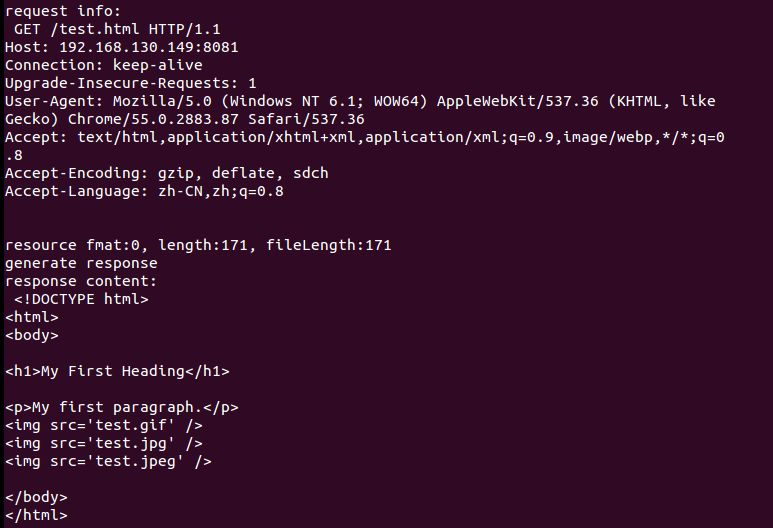
\includegraphics[scale=0.54]{HTML_test.jpg}

\noindent The request message is displayed in the beginning. The first line is the request line, which specifies the method "GET", the URI "/test.html", and the HTTP version. It is asking for a file with the URI specified. The second line is the address of server host. The third line specifies the current connection type. The fourth line suggests that the browser prefer to redirect to an HTTPS connection. The fifth line tells the information of the user. The sixth, seventh, and eighth line lists the acceptable types, encoding and language of the response respectively.\\\\

\noindent After the request message is printed, the server starts to output information about the response. For example, the first line in the graph above suggests that the response format is HTML (represented by 0) and the length of the file is 147. It also prints out the content of the file.\\\\

\noindent After the HTML file is sent, the browser parses the file, finds the references, and places three more requests. The console output for those three are:

\noindent 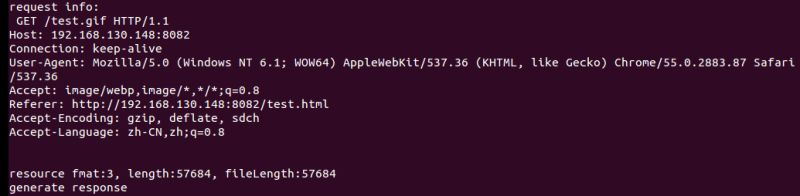
\includegraphics[scale=0.54]{GIF_test.jpg}\\
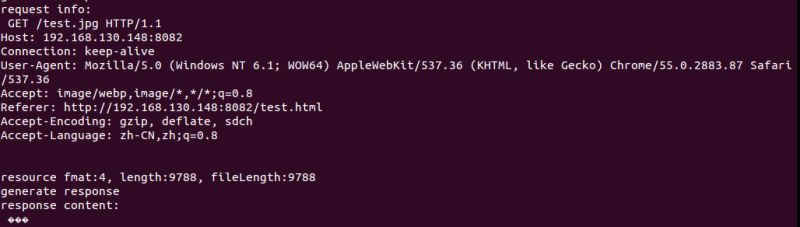
\includegraphics[scale=0.54]{JPG_test.jpg}\\
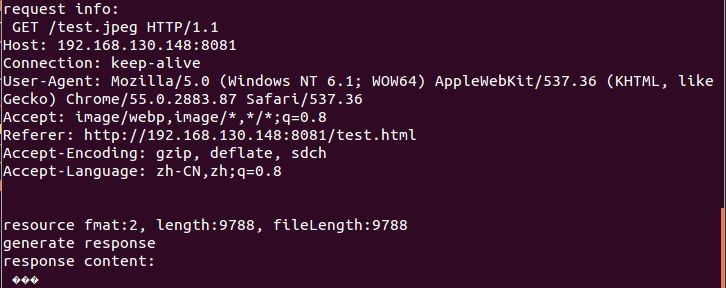
\includegraphics[scale=0.54]{JPEG_test.jpg}\\

\noindent Those request lines are mostly in the same format as in the HTML case, besides that they include a new line to suggest that they are referred by the previous HTML file, and do not inlcude the line for requesting a redirection to HTTPS.


%------------------------------------------------

\section*{Conclusion}

This project implementation meets all the requirements in part A and part B successfully. The web server gives us a better understanding on the client-server model and socket programming with the libraries. It also illustrates an example for HTTP request and response. Though the functionality of the server is simple, it does cover the important concepts, like port, socket, HTTP messages, and etc.

\end{document}